% Created 2024-02-03 Sat 13:50
% Intended LaTeX compiler: pdflatex
\documentclass[11pt]{article}
\usepackage[utf8]{inputenc}
\usepackage[T1]{fontenc}
\usepackage{graphicx}
\usepackage{longtable}
\usepackage{wrapfig}
\usepackage{rotating}
\usepackage[normalem]{ulem}
\usepackage{amsmath}
\usepackage{amssymb}
\usepackage{capt-of}
\usepackage{hyperref}
\usepackage{placeins}
\usepackage{gensymb}
\usepackage{tabularx}
\author{Christian Johnson\and Dan Nusraty\and Dylan Mcgill\and\newline Mailroom 2.0}
\date{\today}
\title{Mail Database Project}
\hypersetup{
 pdfauthor={Christian Johnson\and Dan Nusraty\and Dylan Mcgill\and\newline Mailroom 2.0},
 pdftitle={Mail Database Project},
 pdfkeywords={},
 pdfsubject={},
 pdfcreator={Emacs 28.2.50 (Org mode 9.7-pre)}, 
 pdflang={English}}
\begin{document}

\maketitle
\section{Contents}
\label{sec:orgec19e59}
\subsection{Functional Requirements}
\label{sec:org3a002d0}
\subsection{Non Functional Requirements}
\label{sec:orgaca0829}
\subsection{Use Case Diagram}
\label{sec:org59bcac8}
\subsection{Meeting Summaries}
\label{sec:org3159ffc}
\subsection{Individual Use Cases}
\label{sec:org683ef4c}
\subsubsection{Dan}
\label{sec:org0db10bf}
\subsubsection{Christian}
\label{sec:org7781afb}
\subsubsection{Dylan}
\label{sec:org080ec2a}
\clearpage
\section*{Functional Requirements}
\label{sec:orgb8b3089}
\begin{itemize}
\item Accept data entry
\item Record tracking number and addressed box number for incoming packages
\item Add entered information into sql database
\item Associate incoming packages with Cadet information based on addressed box number
\item Notify Cadet upon package arrival
\item Record package status (Picked up or not)
\item Search database for packages
\item Display all packages matching search terms
\item Easily update package status
\item Developers will write code in an organized fashion, such that the system is easy to expand later.
\end{itemize}
\section*{Non Functional Requirements}
\label{sec:orgfabef02}
\begin{itemize}
\item Will not misassociate packages
\item Will allow package entry, given necessary data, within 5 seconds
\item Will be easily navigable, with all system functions available within 5 clicks
\item Will allow package retrieval, given sufficient search information, within 10 seconds
\item Will never fail to retrieve Cadet information, given sufficient correct search information
\item Will never allow a package entry without associated Cadet information and association
\end{itemize}
\section*{Use Case Diagram}
\label{sec:org29848ab}

\begin{figure}[htbp]
\centering
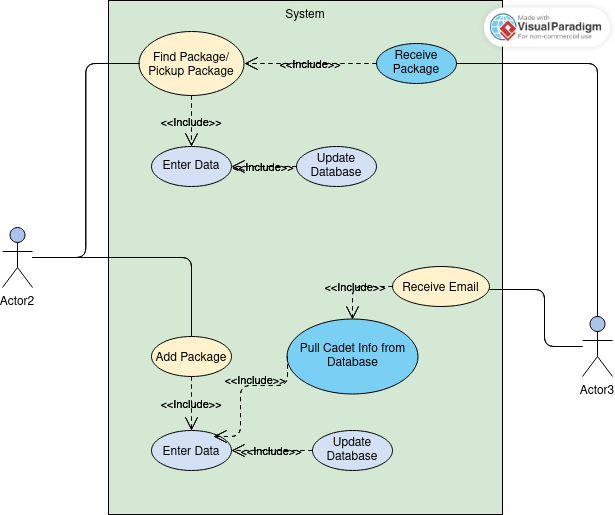
\includegraphics[width=.9\linewidth]{/home/csj7701/Projects/Mail-Database-Project/Class-Documents/Requirements_UseCaseDiagram.png}
\bicaption{.                        Actor 2: Employee, Actor 3: Cadet }
\end{figure}
\newpage
\section*{Meeting Summaries}
\label{sec:org9639d6a}
\subsection*{Meeting 1 - 30JAN2024}
\label{sec:org8b4dc90}
\begin{itemize}
\item Decided on division of labor
\item Agreed on general project scope
\item Began formulating Functional Requirements
\end{itemize}
\subsection*{Meeting 2 - 01FEB2024}
\label{sec:org1b1fbf1}
\begin{itemize}
\item Created Use-Case Diagram
\item Finished Functional Requirements
\item Started Non Functional
\item Started individual Use Cases
\end{itemize}
\subsection*{Meeting 3 - 02FEB2024}
\label{sec:org0148022}
\begin{itemize}
\item Polished Use-Case Diagram
\item Completed Requirements
\item Finished Individual Components
\end{itemize}
\section*{Individual Use Cases}
\label{sec:org8335333}

% DAN

% CHRISTIAN

\begin{table}[tbp]
\hskip-3.0cm\begin{tabularx}{1.5\textwidth}{|X|X|}
\hline
\multicolumn{2}{|c|}{UC02 - Find Package (Christian)} \\
\hline
Scope & SQL Mail Database \\
\hline
Level & User Goal \\
\hline
\Primary Actor & Mailroom Staff \\
\hline
\stakeholders and Interests & Mailroom Staff: Want effificient and simple query methods \\ & Cadets: Want staff to find their package quickly \\
\hline
Precondition & Mailroom has package \\ & Package properly stored in database \\ & Mailroom has correct Cadet info for search \\
\hline
Postconditions & Package information updated in database \\
\hline
Main Success Scenario & 1. Cadet arrives at mailroom \\ &
2. Mailroom staff enters Cadet info \\ & 3. all relevant results are displayed \\
& 4. Mailroom staff retrieves package \\ & 5. Cadet receives package and leaves \\
& 6. Database updated \\
\hline
Extensions & 3a. No results, mailroom staff checks the email sent to the cadet (should contain information to find the package manually) \\
\hline
Special Requirements & None \\
\hline Technology and Data & None \\
\hline Frequency & Nearly Continuous \\
\hline Open Issues & None \\
\hline \end{tabularx} \end{table}

% DYLAN

\begin{table}[tbp]
\vskip-2.0cm\hskip-3.0cm\begin{tabularx}{1.5\textwidth}{|X|X|}
\hline
\multicolumn{2}{|c|}{UC03 - Add Package (Dylan)} \\
\hline
Scope & SQL Mail Database \\
\hline
Level & System goal \\
\hline
Primary Actor & Mailroom Staff \\
\hline
Stakeholders and Interests & Mailroom Staff: Want efficient and streamlined storage of packages \\
 & Cadet: Wants timely and accurate notification of package receipt \\
\hline
Precondition & Package has been physically received by the mailroom staff \\
\hline
Postconditions & Package information has been added to SQL Database \\
 & Email notification has been sent to Cadet \\
 & Package has been stored appropriately \\
\hline
Main Success Scenario & 1. Mailroom staff scans the package \\
 & 2. Automated system scans the package and reads tracking number/box number \\
 & 3: Package status is updated in database along with timestamp and date \\
 & 4. System generates and sends an email to Cadet \\
 & 5. Staff stores the package in appropriate area/box number \\
\hline
Extensions & 1a. Invalid/incomplete information \\
 & 1. Mailroom staff notified, providing option to manually input information \\
 & 3a. Database upload failure \\
 & 3. Mailroom staff notified, given guidance on resolving the issue \\
 & 4a. Email notification failure \\
 & 4. Mailroom staff notified, given guidance on resolving the issue \\
 & Cancel Operation: Mailroom staff may cancel the operation at anytime \\
\hline
Special Requirements & Secure database is used to protect cadet security \\
\hline
Technology and Data & {empty} \\
\hline
Variations List & 1a. Automated scanning system \\
 & 3a. SQL Database \\
 & 4a. Email notification system \\
\hline
Frequency of Occurrence & Regularly: Anytime the mailroom receives a package \\
\hline
Open Issues & Ensure seamless integration with current scanners \\
 & User training \\
 & Systems ability to handle high volume of packages during highly busy times \\
\hline
\end{tabularx}
\end{table}
\end{document}